\documentclass[tikz,border=4pt]{standalone}
% Shared style for every figure and for the deck: one accent, one
% highlight, thin lines, rounded nodes, nothing decorative.
\usepackage[T1]{fontenc}
\usepackage{lmodern}
\renewcommand{\familydefault}{\sfdefault}
\usepackage{tikz}
\usetikzlibrary{arrows.meta,positioning,calc,shapes.misc,fit,backgrounds,decorations.pathreplacing}
\definecolor{ink}{RGB}{40,40,40}
\definecolor{soft}{RGB}{150,150,150}
\definecolor{faint}{RGB}{225,225,225}
\definecolor{accent}{RGB}{0,95,115}
\definecolor{accentlight}{RGB}{214,232,236}
\definecolor{warn}{RGB}{196,84,40}
\definecolor{warnlight}{RGB}{247,226,216}
\tikzset{
  every picture/.style={color=ink, line width=0.5pt, font=\small},
  node distance=12mm and 18mm,
  box/.style={draw=ink, rounded corners=2pt, fill=white, inner sep=5pt, minimum height=7mm, align=center},
  maker/.style={box, minimum width=18mm},
  cat/.style={box, inner sep=3.5pt, minimum height=6mm},
  root/.style={box, fill=accentlight, draw=accent},
  bad/.style={box, fill=warnlight, draw=warn},
  ghost/.style={box, draw=soft, text=soft, dashed},
  flow/.style={-{Stealth[length=4pt,width=3.5pt]}, line width=0.5pt},
  sub/.style={-{Stealth[length=4pt,width=3.5pt]}, line width=0.5pt, color=soft},
  strong/.style={flow, color=accent, line width=0.8pt},
  wrong/.style={flow, color=warn},
  lbl/.style={font=\footnotesize, text=ink, inner sep=1.5pt, fill=white},
  note/.style={font=\footnotesize, text=soft, align=center},
  rate/.style={font=\footnotesize, text=accent, inner sep=1pt, fill=white},
}

\usepackage{amsmath}
\usepackage{pgfplots}
\pgfplotsset{compat=1.17}

\begin{document}
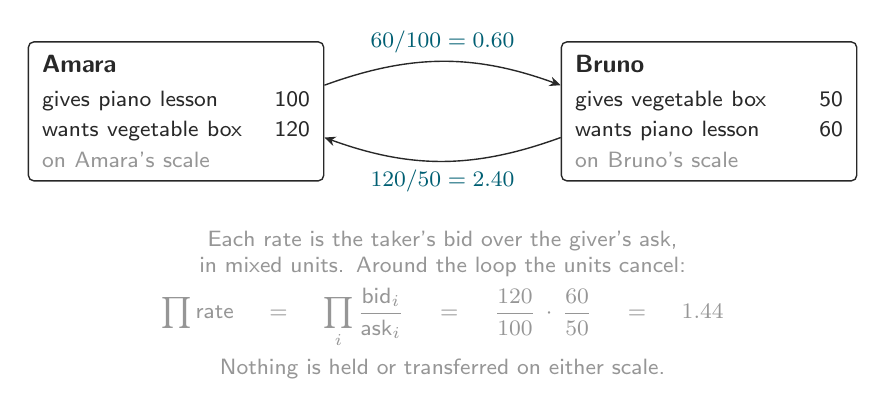
\begin{tikzpicture}
  \node[maker, align=left, text width=34mm] (A) {\textbf{Amara}\\[1pt]{\footnotesize gives piano lesson \hfill 100}\\{\footnotesize wants vegetable box \hfill 120}\\{\footnotesize\color{soft}on Amara's scale}};
  \node[maker, align=left, text width=34mm, right=30mm of A] (B) {\textbf{Bruno}\\[1pt]{\footnotesize gives vegetable box \hfill 50}\\{\footnotesize wants piano lesson \hfill 60}\\{\footnotesize\color{soft}on Bruno's scale}};
  \draw[flow] (A.10) to[bend left=20] node[rate, above=2pt] {$60/100 = 0.60$} (B.170);
  \draw[flow] (B.190) to[bend left=20] node[rate, below=2pt] {$120/50 = 2.40$} (A.-10);
  \node[note, anchor=north, text width=92mm] at ($(A.south)!0.5!(B.south) + (0,-5mm)$) {Each rate is the taker's bid over the giver's ask, in mixed units. Around the loop the units cancel:\\[3pt] $\displaystyle \prod \text{rate} \;=\; \prod_i \frac{\text{bid}_i}{\text{ask}_i} \;=\; \frac{120}{100}\cdot\frac{60}{50} \;=\; 1.44$\\[3pt] Nothing is held or transferred on either scale.};
\end{tikzpicture}
\end{document}
